\documentclass[12pt]{article}
%\usepackage[utf8]{inputenc}
%\documentclass[UTF8]{ctexart}
%\usepackage[UTF8, heading = false, scheme = plain]{ctex}
\usepackage{geometry}
%geometry{a4paper,scale=0.9}
\geometry{a4paper,left=1cm,right=1cm,top=1cm,bottom=2cm}
\usepackage{amsfonts}
\usepackage{color}
\usepackage{url}
%\usepackage{biblatex}
\usepackage{amsmath}
\usepackage{amssymb}
\usepackage{latexsym}
\usepackage{cite}
%\addbibresource{ref.bib}
%\bibliography{ref.bib}
\usepackage{caption}
\usepackage{graphicx, subfig}
\usepackage{float}
%\usepackage[fontset=ubuntu]{ctex}
%\usepackage{fontspec}
\usepackage{xeCJK}
%\usepackage[colorlinks,
%anchorcolor=black,
%citecolor=black]{hyperref}
%\setmainfont{SimSun}
\usepackage[section]{placeins}
\usepackage{enumitem}
\usepackage{framed}
\usepackage[framemethod=TikZ]{mdframed}
\usepackage{indentfirst}
\usepackage{setspace}%使用间距宏包
\linespread{1.5}

\title{K8s}
\author{leolinuxer}
%\date{June 2020}

\begin{document}
%\setlength{\parindent}{0pt}
\maketitle
\tableofcontents

\section{背景}
\url{https://zhuanlan.zhihu.com/p/103124918}

k8s全称kubernetes。k8s是为容器服务而生的一个可移植容器的编排管理工具,越来越多的公司正在拥抱k8s,并且当前k8s已经主导了云业务流程,推动了微服务架构等热门技术的普及和落地,正在如火如荼的发展。

首先,我们从容器技术谈起,在容器技术之前,大家开发用虚拟机比较多,比如vmware和openstack,我们可以使用虚拟机在我们的操作系统中模拟出多台子电脑(Linux),子电脑之间是相互隔离的,但是虚拟机对于开发和运维人员而言,存在启动慢,占用空间大,不易迁移的缺点。举一个我亲身经历过的场景吧,之前在vmware中开发了一个线下平台,为了保证每次能够顺利使用,我们就把这个虚拟机导出为OVF,然后随身携带,用的时候在服务器中部署,这里就充分体现了虚拟机的缺点。

接着,容器化技术应运而生,它不需要虚拟出整个操作系统,只需要虚拟一个小规模的环境即可,而且启动速度很快,除了运行其中应用以外,基本不消耗额外的系统资源。Docker是应用最为广泛的容器技术,通过打包镜像,启动容器来创建一个服务。但是随着应用越来越复杂,容器的数量也越来越多,由此衍生了管理运维容器的重大问题,而且随着云计算的发展,云端最大的挑战,容器在漂移。在此业务驱动下,k8s问世,提出了一套全新的基于容器技术的分布式架构领先方案,在整个容器技术领域的发展是一个重大突破与创新。

那么,K8S实现了什么?

从架构设计层面,我们关注的可用性,伸缩性都可以结合k8s得到很好的解决,如果你想使用微服务架构,搭配k8s,真的是完美,再从部署运维层面,服务部署,服务监控,应用扩容和故障处理,k8s都提供了很好的解决方案。

具体来说,主要包括以下几点:
\begin{itemize}
\setlength{\itemsep}{0pt}
\setlength{\parsep}{0pt}
\setlength{\parskip}{0pt}
    \item 服务发现与调度
    \item 负载均衡
    \item 服务自愈
    \item 服务弹性扩容
    \item 横向扩容
    \item 存储卷挂载
\end{itemize}

总而言之,k8s可以使我们应用的部署和运维更加方便。

\section{K8s 架构}
最后,我们看下k8s的架构:
\begin{figure}[H]
    \centering
    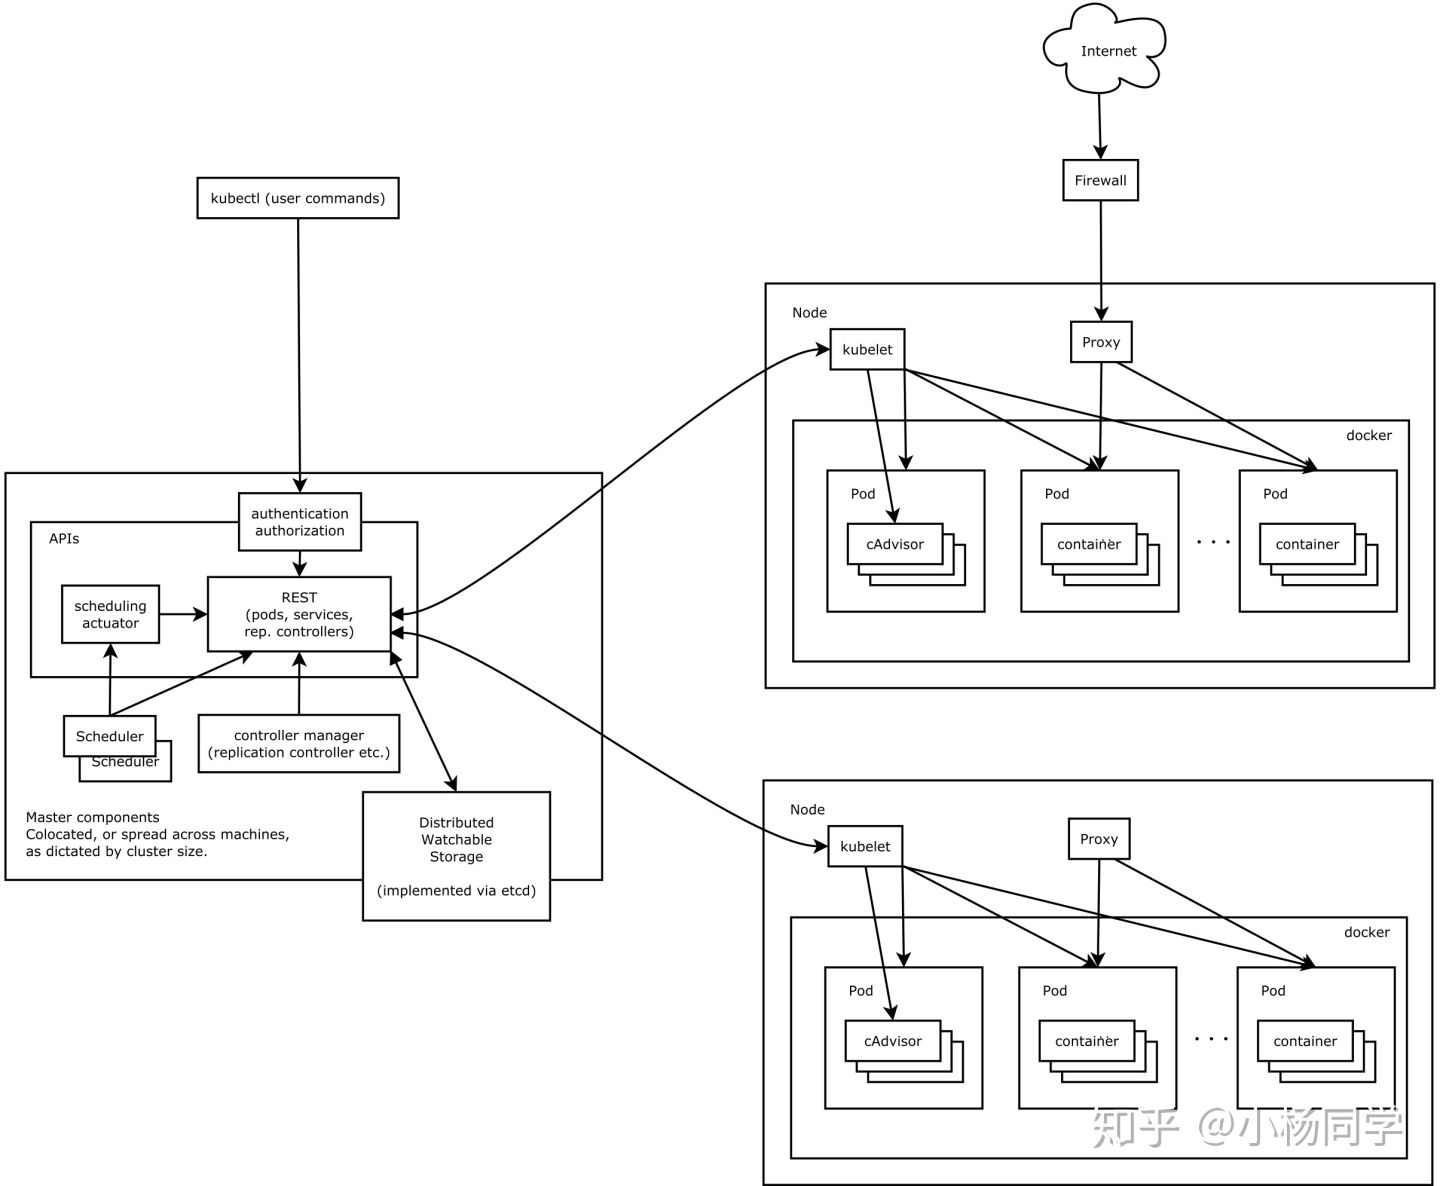
\includegraphics[width=1\textwidth]{fig/K8s_Structure.jpg}
\end{figure}

k8s集群由Master节点和Node(Worker)节点组成。

\subsection{Master 节点}
Master节点指的是集群控制节点,管理和控制整个集群,基本上k8s的所有控制命令都发给它,它负责具体的执行过程。在Master上主要运行着:

\begin{enumerate}
\setlength{\itemsep}{0pt}
\setlength{\parsep}{0pt}
\setlength{\parskip}{0pt}
    \item Kubernetes Controller Manager(kube-controller-manager):k8s中所有资源对象的自动化控制中心,维护管理集群的状态,比如故障检测,自动扩展,滚动更新等。
    \item Kubernetes Scheduler(kube-scheduler): 负责资源调度,按照预定的调度策略将Pod调度到相应的机器上。
    \item etcd:保存整个集群的状态。
\end{enumerate}

\subsection{Worker 节点}
除了master以外的节点被称为Node或者Worker节点,可以在master中使用命令 kubectl get nodes查看集群中的node节点。每个Node都会被Master分配一些工作负载(Docker容器),当某个Node宕机时,该节点上的工作负载就会被Master自动转移到其它节点上。在Node上主要运行着:
\begin{enumerate}
\setlength{\itemsep}{0pt}
\setlength{\parsep}{0pt}
\setlength{\parskip}{0pt}
    \item kubelet:负责Pod对应的容器的创建、启停等任务,同时与Master密切协作,实现集群管理的基本功能。
    \item ube-proxy:实现service的通信与负载均衡。
    \item docker(Docker Engine):Docker引擎,负责本机的容器创建和管理。
\end{enumerate}

\subsection{pod —— k8s 调度的最小单元}
\url{https://www.jianshu.com/p/502544957c88}

一个 pod 包含一组容器,一个 pod 不会跨越多个工作节点
\begin{itemize}
\setlength{\itemsep}{0pt}
\setlength{\parsep}{0pt}
\setlength{\parskip}{0pt}
    \item pod 相当于逻辑主机,每个 pod 都有自己的 IP 地址
    \item pod 内的容器共享相同的 IP 和端口空间
    \item 默认情况下,每个容器的文件系统与其他容器完全隔离
\end{itemize}






%\printbibliography
\bibliography{../ref}
\bibliographystyle{IEEEtran}
\end{document}